% 


\documentclass[twoside]{article}
\setlength{\oddsidemargin}{0.25 in}
\setlength{\evensidemargin}{-0.25 in}
\setlength{\topmargin}{-0.6 in}
\setlength{\textwidth}{6.5 in}
\setlength{\textheight}{8.5 in}
\setlength{\headsep}{0.75 in}
\setlength{\parindent}{0 in}
\setlength{\parskip}{0.1 in}

%
% ADD PACKAGES here:
%

\usepackage{amsmath,amsfonts,graphicx,arydshln}


\newcounter{lecnum}
\renewcommand{\thepage}{\thelecnum-\arabic{page}}
\renewcommand{\thesection}{\thelecnum.\arabic{section}}
\renewcommand{\theequation}{\thelecnum.\arabic{equation}}
\renewcommand{\thefigure}{\thelecnum.\arabic{figure}}
\renewcommand{\thetable}{\thelecnum.\arabic{table}}

%
% The following macro is used to generate the header.
%
\newcommand{\lecture}[4]{
   \pagestyle{myheadings}
   \thispagestyle{plain}
   \newpage
   \setcounter{lecnum}{#1}
   \setcounter{page}{1}
   \noindent
   \begin{center}
   \framebox{
      \vbox{\vspace{2mm}
    \hbox to 6.28in { {\bf EE502 - Linear Systems Theory II
	\hfill Spring 2023} }
       \vspace{4mm}
       \hbox to 6.28in { {\Large \hfill Lecture #1 \hfill} }
       \vspace{2mm}
       \hbox to 6.28in { {\it Lecturer: #2 \hfill } }
      \vspace{2mm}}
   }
   \end{center}
   \markboth{Lecture #1}{Lecture #1}

   \vspace*{4mm}
}

\renewcommand{\cite}[1]{[#1]}
\def\beginrefs{\begin{list}%
        {[\arabic{equation}]}{\usecounter{equation}
         \setlength{\leftmargin}{2.0truecm}\setlength{\labelsep}{0.4truecm}%
         \setlength{\labelwidth}{1.6truecm}}}
\def\endrefs{\end{list}}
\def\bibentry#1{\item[\hbox{[#1]}]}


\newcommand{\fig}[3]{
			\vspace{#2}
			\begin{center}
			Figure \thelecnum.#1:~#3
			\end{center}
	}

% Use these for theorems, lemmas, proofs, etc.
\newtheorem{theorem}{Theorem}[lecnum]
\newtheorem{lemma}[theorem]{Lemma}
\newtheorem{proposition}[theorem]{Proposition}
\newtheorem{claim}[theorem]{Claim}
\newtheorem{corollary}[theorem]{Corollary}
\newtheorem{definition}[theorem]{Definition}
\newenvironment{proof}{{\bf Proof:}}{\hfill\rule{2mm}{2mm}}
\newtheorem{exmp}[theorem]{Ex}

% **** IF YOU WANT TO DEFINE ADDITIONAL MACROS FOR YOURSELF, PUT THEM HERE:

\begin{document}

% Lecture Details
\lecture{14}{Asst. Prof. M. Mert Ankarali}

%%%%%%%%%%%%%%%%%%%%%%%%%%

\section{State Observer}

Generally the full state measurment,$x(t)$ or $x[k]$, of a system is not accessible and \textit{observers, estimators, filters})
have to be used to extract this information. The output, $y(t)$ or $y[k]$, represents the actual measurements
which is a function of the input and the output. We will mainly focus on DT systems in this lecture however, 
all of the derivations and concepts are either same with the CT case or can be easily adopted with minor modifications. Let 
%
\begin{align*}
  x[k+1] &= A x[k] + B u[k]
  \\
  y[k] &= C x[k] + D u[k]
\end{align*}
%
A Luenberger observer is built using a ``simulated'' model of the 
system and the errors caused by the mismatched initial conditions 
$x_0 \neq \hat{x}_0$ (or other types of perturbations)
are reduced by introducing output error feedback.

Let's assume that the state vector of the simulated system
is $\hat{x}[k]$, then the state space equation of this
synthetic system takes the form
%
\begin{align*}
  \hat{x}[k+1] &= A \hat{x}[k] + B u[k]
  \\
  \hat{y}[k] &= C \hat{x}[k] + D u[k]
\end{align*}
%
Note that since $u[k]$ is the input that is supplied by the 
controller, we assume that it is known apriori. If $x[0] = \hat{x}[0]$ and
when there is no model mismatch or uncertainty in the system
then we expect that $x[k] = \hat{x}[k]$ and $y[k] = \hat{y}[k]$ 
for all $k$. When $x[0] \neq \hat{x}[0]$, then we should observe a 
difference between the measured and predicted output
$y[k] \neq \hat{y}[k]$. The core idea in Luenberger observer
is feeding the error in the output prediction 
$y[k] - \hat{y}[k]$ to the simulated system via a linear feedback gain.
%
\begin{align*}
  \hat{x}[k+1] &= A \hat{x}[k] + B u[k] + L \left( y[k] - \hat{y}[k] \right) 
  \\
  \hat{y}[k] &= C \hat{x}[k] + D u[k]
\end{align*}
%
In order to understand how a Luenberger observer works and
to choose a proper observer gain $L$, we define an error signal
$e[k] = x[k] - \hat{x}[k]$. The dynamics w.r.t $e[k]$ can be derived
as
%
\begin{align*}
  e[k+1] &= x[k+1] - \hat{x}[k+1]
        \\
     &= \left( A x[k] + B u[k] \right)
  - \left( A \hat{x}[k] + B u[k] + L \left( y[k] - \hat{y}[k] \right)
       \right)
\\
   e[k+1] &= \left( A - L C \right) e[k]
\end{align*}
%
where $e[0] = x[0] - \hat{x}[0]$ denotes the error in the initial
condition. 

If the matrix $\left( A - L C \right)$ is stable then the errors in
initial condition will diminish eventually. Moreover, in order
to have a good observer/estimator performance the observer
convergence should be sufficiently fast. 

\textbf{Theorem: (Observer Eigenvalue Placement)} Given $(A,C)$, $\exists L$ s.t. 
%
\begin{align*}
	\mathrm{det}\left[ \lambda I - (A - L C ) \right] &= \lambda^n + a_{n-1}^*  \lambda^{n-1}
	+ \cdots + a_{1}^* \lambda + a_0^*
	\\
	\forall \mathcal{A} &= \lbrace a_0^* , \, a_1^* \, \cdots \, a_{n-1}^* \rbrace , \, a_i^* \in \mathbb{R}
\end{align*} 
%
if and only if $(A,C)$ is observable. 

\textbf{Proof of necessity: } Let's assume that $(A,C)$ not observable and $\exists (\lambda_u , v_u)$ pair such that
$A v_u = v_u \lambda_u $ and $C v_u = 0$. Now check weather $v_u$ is a right eigenvector of $(A - L C)$
%
\begin{align*}
	 (A - L C ) v_u &= A v_u - L C v_U = A v_u = \lambda_u v_U
	\\
        C v_u  &= 0
\end{align*} 
%
Here not only we showed that $\lambda_u$ can not be moved hence it is not possible to locate the observer poles to
arbitrary locations, we also showed that state-observer rule does not affect the observability.

\textbf{Proof of sufficiency:} Note that if $(A,C)$ pair is observable then $(A^T,C^T)$ pair is reachable. Then we know that 
$\exists L^T$ s.t. 
%
\begin{align*}
	\mathrm{det}\left[ \lambda I - (A^T - C^T L^T ) \right] &= \lambda^n + a_{n-1}^*  \lambda^{n-1}
	+ \cdots + a_{1}^* \lambda + a_0^* 
	\\
	\forall \mathcal{A} &= \lbrace a_0^* , \, a_1^* \, \cdots \, a_{n-1}^* \rbrace , \, a_i^* \in \mathbb{R}
\end{align*} 
%
and obviously 
%
\begin{align*}
	\mathrm{det}\left[ \lambda I - (A^T - C^T L^T ) \right] &= \mathrm{det}\left[ \lambda I - (A - L C ) \right] 
\end{align*} 
%
which completes the proof.

\section{Detectability}

The dual of stabilizability in the observability domain is called detectability. 

\textbf{Theorem} The following statements are equal 
\begin{itemize}
\item $(A,C)$ is detectable $\iff$
\item if unobservable modes of $(A,C)$ are asymptotically stable $\iff$
\item $\forall (\lambda_i , v_i)$ s.t. $A v_i = \lambda_i v_i$ $\iff$
and $\mathrm{Re}\lbrace \lambda_i \rbrace \geq 0$ (or $|\lambda_i|\geq0$),
$v_i \notin \mathcal{N}(C)$ $\iff$
\item $\mathrm{rank}\left[ \begin{array}{c} A - \lambda I \\ \hline C \end{array} \right] = n$,
$\forall \lambda \in \mathbb{C}$ s.t. $\mathrm{Re}\lbrace \lambda_i \rbrace \geq 0$ for CT systems (or $\forall \lambda \in \mathbb{C}$ s.t. $|\lambda|  \geq 1$ for DT systems)
\item $\exists L$ such that $(A - L C)$ is asymptotically stable
\end{itemize}

\newpage

\section{Model Based Controllers: Closing the loop between the observer and state-feedback control low} 

In the state-feedback control policy, we defined the control
law as
%
\begin{align*}
 u[k] = \alpha r[k] - K x[k]
\end{align*}
%
However, as mentioned in the Observer section, in general, we don't have direct access to all states of the system. In this case, we learned how to design an Observer/Estimator that predicts the states of the system. In this respect, it is natural to assume that in a closed-loop system, the control policy that defines the input should depend on the estimated states.
%
\begin{align*}
 u[k] = \alpha r[k] - K \hat{x}[k]
\end{align*}
%
However, the critical question is how this coupling affects the closed-loop behavior, and an even deeper question is can we even use such a policy. The advantage of LTI systems is that state-feedback gain and observer gain can be separately designed, and we guarantee a stable closed-loop performance. In this section, we will analyze the coupled system.
%
Equations of motion for the closed-loop observer \& state-feedback
based control system is given below
%
\begin{align*}
   x[k+1] &= A x[k] + B u[k]
  \\ 
   y[k] &= C x[k] + D u[k]
  \\
  \hat{x}[k+1] &= A \hat{x}[k] + B u[k] + L \left( y[k] - \hat{y}[k] \right) 
  \\
  \hat{y}[k] &= C \hat{x}[k] + D u[k]
  \\
   u[k] &= -K \hat{x}[k]
\end{align*}
%
If we eliminate $u[k]$ and $\hat{y}[k]$ we obtain following 
dynamical representation
%
\begin{align*}
   x[k+1] &= A x[k] - B K \hat{x}[k] + B \alpha r[k]
  \\
  \hat{x}[k+1] &= A \hat{x}[k] - B K \hat{x}[k] + L C \left( x[k] -
                 \hat{x}[k] \right) + B \alpha r[k]
  \\ 
   y[k] &= C x[k] - D K \hat{x}[k] + D \alpha r[k]
\end{align*}
%
Now let's replace $\hat{x}[k]$ with $e[k] = x[k] - \hat{x}[k]$
%
\begin{align*}
   x[k+1] &= ( A - B K ) x[k] + B K e[k] + B \alpha r[k]
  \\
  e[k+1] &= ( A - LC ) e[k]
  \\ 
   y[k] &= (C - D K) x[k] + D K e[k] + D \alpha r[k]
\end{align*}
%
Now let's define a state for the whole system, 
$z[k] = \left[ \begin{array}{c} x[k] \\ e[k] \end{array} \right]$
then the state-space representation is given by
%
\begin{align*}
  z[k+1] = \left[ \begin{array}{cc} (A - B K) & B K\\ 0_{n \times n}
                                              & (A - LC) \end{array}
                                                \right] z[k] + \left[ \begin{array}{c} \alpha B \\ 0 \end{array} \right] r[k]
\\
 y[k] = \left[ \begin{array}{cc} (C - D K) & D K \end{array}
                                                \right] z[k] + [\alpha D] r[k]
\end{align*}
%
The system matrix is in block diagonal form, and the eigenvalues
of this new system, the matrix is found by taking the union of eigenvalues
of $(A - B K)$ and eigenvalues of $(A - L C)$. Thus a separate
pole-placement can be performed for the state-feedback controller
and the observer. 

\begin{exmp}
Consider the following open-loop digital control systems
\end{exmp}

    \begin{center}
  \begin{minipage}[h]{0.9\linewidth}
    \begin{center}
      \includegraphics[width=0.65\textwidth]{block_open-loop}
    \end{center}
  \end{minipage}
    \end{center}

\begin{enumerate}
	\item Find the discrete-time state-space representation between the discrete time input signal, $u[k]$
	and the discrete time output signal, $u[k]$, given that state definition is $x[k] = \begin{bmatrix} x_1[k]  \\ x_2[k] \end{bmatrix}$. Note that
	sampling time is generic for this problem $T$.
	
\vspace{6pt}

\textbf{Solution:} The state update equation of the continuous-time plant has the following form
%
\begin{align*}
 \dot{x} &= A_{ct} x + B_{ct} u \ , \  x(t) = \begin{bmatrix} x_1(t)  \\ x_2(t) \end{bmatrix}
 \\
 A_{ct} &= \begin{bmatrix} 0 & 1 \\ 0 & 0 \end{bmatrix} \ , \ B_{ct} = \begin{bmatrix} 0 \\ 1 \end{bmatrix}
\end{align*}
%
Since the ADC block is a simple ZOH operator we can find the system matrix of the discritized system 
using the state-transitions matrix of the CT-Plant
%
\begin{align*}
 A_{dt} &= e^{A_{ct} T} = I + A_{ct} T + 0 + \cdots
 \\
 &= \begin{bmatrix} 1 & 0 \\ 0 & 1 \end{bmatrix} + \begin{bmatrix} 0 & T \\ 0 & 0 \end{bmatrix} =  \begin{bmatrix} 1 & T \\ 0 & 1 \end{bmatrix}
\end{align*}
%
Since $A_{ct}$ is not invsertable, we need to derive $B_{dt}$ using the following relation
%
%
\begin{align*}
 B_{dt} &= \int\limits_{0}^{T} e^{A_{ct} \tau} B_{ct} d\tau = 
 \int\limits_{0}^{T}  \begin{bmatrix} 1 & \tau \\ 0 & 1 \end{bmatrix} \begin{bmatrix} 0 \\ 1 \end{bmatrix}  d\tau = 
 \int\limits_{0}^{T}  \begin{bmatrix} \tau \\ 1 \end{bmatrix}  d\tau = 
 \begin{bmatrix} T^2/2 \\ T \end{bmatrix} 
\end{align*}
%
Output equation is simply equal to $y[k] = x_1[k]$, and thus $C_{dt} = C_{ct} = C = \begin{bmatrix} 1 & 0 \end{bmatrix} $
and $D_{dt} = D_{ct} = CD= \begin{bmatrix} 0 \end{bmatrix} $.

\item Show that following closed-loop PD type controller is indeed a form of state-feedback rule
		
\begin{center}
  \begin{minipage}[h]{0.9\linewidth}
    \begin{center}
      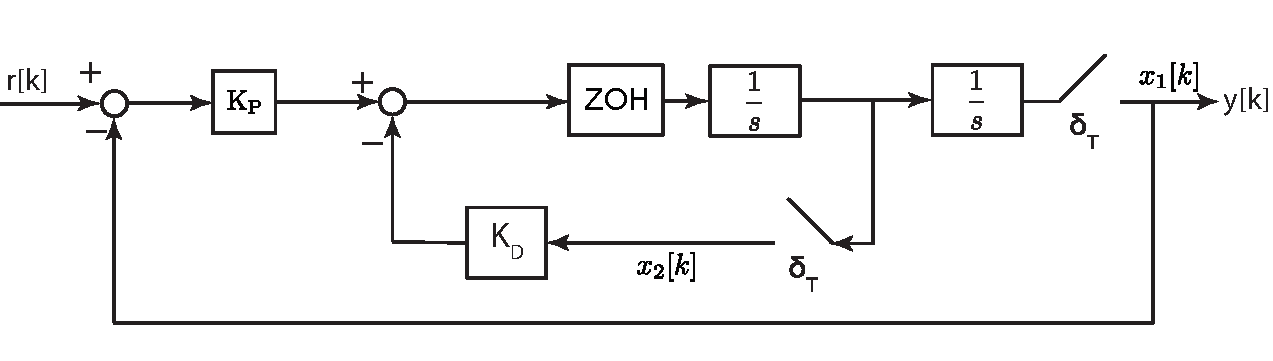
\includegraphics[width=0.9\textwidth]{block_PD}
    \end{center}
  \end{minipage}
    \end{center}
		
\textbf{Solution:} Let's explicitly write $u[k]$
%
\begin{align*}
u[k] &= K_P (r[k] - x_1[k]) + K_D x_2[k] = K_P r[k] - \begin{bmatrix} K_P & K_D \end{bmatrix} x[k] \\
K &= \begin{bmatrix} K_P & K_D \end{bmatrix} \ , \ \alpha = K_P
\end{align*}
%
\item Show that we can always find a $(K_P,K_D)$ pair such that closed-loop poles are located
at arbitrary desired locations. 

\textbf{Solution:} We need to simply show that $(A_{dt} , B_{dt})$ pair is reachable
%
\begin{align*}
\mathbf{R} = \left[ \begin{array}{c|c} A_{dt} B_{dt} & B_{dt} \end{array} \right] = 
\left[ \begin{array}{c|c} 3 T^2 /2 & T^2/2 \\ T & T \end{array} \right] \, \Rightarrow \, \mathrm{rank}[\mathbf{R}] = 2  
\end{align*}
%
thus $(A_{dt} , B_{dt})$ reachable and it implies that we can always find a $(K_P,K_D)$ pair such that closed-loop poles are located
at arbitrary desired locations. 

\item Find $(K_P,K_D)$ such that closed-loop systems shows dead-beat behavior

\textbf{Solution:} In such a case, we need to place the closed-loop eigenvalues at the origin 
%
\begin{align*}
	A_{cl} &= A_{dt} - B_{dt} K =  \begin{bmatrix} 1 & T \\ 0 & 1 \end{bmatrix} - \begin{bmatrix} T^2/2 \\ T \end{bmatrix} 
	\begin{bmatrix} K_P & K_D \end{bmatrix} 
	=  \begin{bmatrix} 1 & T \\ 0 & 1 \end{bmatrix} -  \begin{bmatrix} K_P T^2/2  & K_D T^2/2 \\ K_P T & K_D T \end{bmatrix}  
	\\
	&=  \begin{bmatrix} 1 - K_P T^2/2  & T - K_D T^2/2 \\ - K_P T & 1 - K_D T \end{bmatrix}
	\\
	\lambda I - A_{cl} &= \begin{bmatrix} \lambda - 1 + K_P T^2/2  & - T + K_D T^2/2 \\  K_P T & \lambda -  1+ K_D T \end{bmatrix}
	\\
	\mathrm{det}\left( \lambda I - A_{cl} \right) &= \lambda^2 + \left( K_P T^2/2 + K_D T - 2 \right) \lambda + \left( K_P T^2/2 - K_D T + 1 \right)
	\\
	\begin{bmatrix} 2 \\ -1 \end{bmatrix} 
	&= \begin{bmatrix} T^2/2 & T \\ T^2/2 & -T \end{bmatrix} \begin{bmatrix} K_P \\ K_D \end{bmatrix} 
	\, \Rightarrow \, \begin{bmatrix} K_P \\ K_D \end{bmatrix} = \frac{1}{T} \begin{bmatrix} T/2 & 1 \\ T/2 & -1 \end{bmatrix}^{-1}  \begin{bmatrix} 2 \\ -1 \end{bmatrix} =  \frac{1}{T} \begin{bmatrix} 1/T & 1/T \\ 1/2 & -1/2 \end{bmatrix} \begin{bmatrix} 2 \\ -1 \end{bmatrix} 
	\\
	\begin{bmatrix} K_P \\ K_D \end{bmatrix} &= \begin{bmatrix} 1/T^2 \\ 3/(2 T) \end{bmatrix}
	\, \Rightarrow \, K =  \begin{bmatrix} 1/T^2 & 3/(2 T) \end{bmatrix}
	\\
	A_{cl} &= \begin{bmatrix} 1/2 & T/4 \\ -1/T & -1/2  \end{bmatrix}
\end{align*}

\item Now design observer as shown in the figure below such that the observer states converge the actual state in a deadbeat fashion.
		
\begin{center}
  \begin{minipage}[h]{0.9\linewidth}
    \begin{center}
      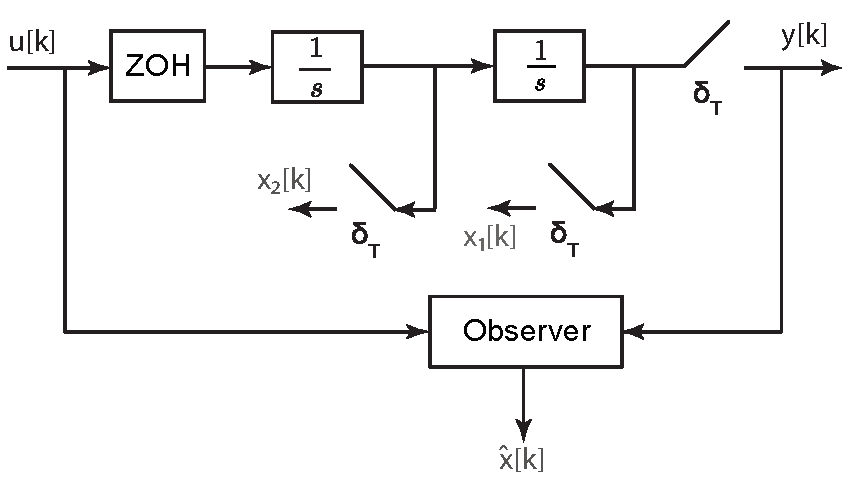
\includegraphics[width=0.75\textwidth]{block_open-loop-obs}
    \end{center}
  \end{minipage}
    \end{center}

\textbf{Solution:} Let's first check weather the system is observable or not
%
\begin{align*}
\mathbf{O} = \left[ \begin{array}{cc} C \\ \hline C A_{dt} \end{array} \right] =
\left[ \begin{array}{cc} 1 & 0 \\ \hline 1 & T \end{array} \right]
\ , \ \mathrm{rank}( \mathbf{O} ) = 2 \, \Rightarrow \, \mathrm{observable}
\end{align*}
%
Now let's design the observer. We know that observer's state-space model has the following form
%
\begin{align*}
  \hat{x}[k+1] &= A_{dt} \hat{x}[k] + B_{dt} u[k] + L \left( y[k] - C \hat{x}[k] \right) 
\end{align*}
%
and the error dynamics between the actual and predicted states has the following autonomous structure
%
\begin{align*}
  e[k+1] &= ( A_{dt} - LC ) e[k]
\end{align*}
%
In order to obtain dead-beat behavior in error dynamics 
%
\begin{align*}
  \mathrm{det}( \lambda I -  A_o ) &= \lambda^2 \ , \ A_{o} = ( A_{dt} - LC )
  \\
  ( \lambda I -  A_o ) &= \begin{bmatrix} \lambda & 0 \\ 0 & \lambda \end{bmatrix} - \begin{bmatrix} 1 & T \\ 0 & 1 \end{bmatrix} 
  + \begin{bmatrix} l_1 \\ l_2 \end{bmatrix} \begin{bmatrix} 1 & 0 \end{bmatrix} 
  = \begin{bmatrix} \lambda - 1 + l_1 & -T \\ l_2 & \lambda - 1 \end{bmatrix} 
  \\
   \mathrm{det}( \lambda I -  A_o ) &= \lambda^2 + ( l_1 - 2 ) \lambda + ( -l_1 + T l_2 + 1 ) 
   \\
   L &= \begin{bmatrix} l_1 \\ l_2 \end{bmatrix} = \begin{bmatrix} 2 \\ 1/T \end{bmatrix} \, \Rightarrow \, A_o = \begin{bmatrix} -1 & T \\ -1/T & 1 \end{bmatrix} 
\end{align*}

\item Now close the loop using the observers estimated states as shown i the figure below. Fine the state-space representation of the whole closed-loop system 
and comment on the transient behavior of the dynamics

\begin{center}
  \begin{minipage}[h]{0.9\linewidth}
    \begin{center}
      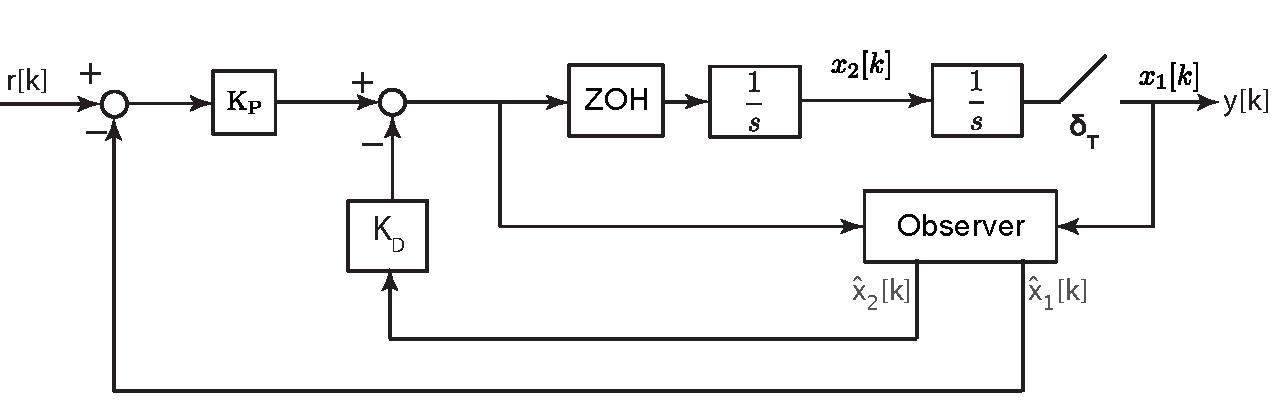
\includegraphics[width=0.95\textwidth]{block_PD_obs}
    \end{center}
  \end{minipage}
    \end{center}

\textbf{Solution:} In the lecture notes for a closed-loop observer and state-feedback structure, we already derived the full state-space form
 %
\begin{align*}
  z[k+1] &= \left[ \begin{array}{cc} (A_{dt} - B_{dt} K) & B_{dt} K\\ 0_{n \times n}
                                              & (A_{dt} - LC) \end{array}
                                                \right] z[k] + \left[ \begin{array}{c} \alpha B_{dt} \\ 0 \end{array} \right] r[k]
\ , \
 y[k] = \left[ \begin{array}{cc} C & 0  \end{array}
                                                \right] z[k]  
                                                \\
  z[k+1] &= \left[ \begin{array}{cc|cc} 1/2 & T/4 & K_P T^2/2 & K_D T^2/2 \\ -1/T & -1/2 & K_P T & K_D T \\ \hline 0 & 0 & -1 & T \\ 0 & 0 & -1/T & 1 \end{array}
                                                \right] z[k] + \left[ \begin{array}{c} K_P T^2/2 \\ K_P T \\ \hline 0 \\ 0 \end{array} \right] r[k]                                              
\end{align*}
%



\end{enumerate}


% **** This ENDS THE EXAMPLES. DON'T DELETE THE FOLLOWING LINE:
\end{document}
